\section{Calorimeter Noise simulation}
\label{sc:CaloNoise}

Fluctuations in the calorimeter electronics noise can be a source of a small amount of missing energy. Therefore, the first step
in making comparisons between Monte Carlo simulation and data is to look at the detector noise and its simulation. For this purpose
events from the following two samples were used:

\begin{itemize}
  \item Noise-only sample: \newline
This sample was produced in CMSSW\_3\_3\_6\_path3 by generating single electron neutrinos with the rest of the configuration identical to the one used to
produce /MinBias/Summer09-STARTUP3X\_V8P\_900GeV-v1/GEN-SIM-RECO dataset. No special event selection was applied.

  \item /ZeroBias/BeamCommissioning09-Jan23ReReco-v1/RECO: \newline
Events selected from this dataset were required to pass the veto on TT bit 0, i.e., bunch crossings corresponding to the beam-beam
collisions were excluded from the selection. Events selected in this way are almost completely noise-dominated.
\end{itemize}

Figure~\ref{fig:subdet_RecHitE} shows the comparison between RecHit energy distributions in noise-only and selected ZeroBias data for different
calorimeter sub-detectors. Figure~\ref{fig:subdet_CaloSumET} shows the comparison between CaloSumET distributions in noise-only and selected 
ZeroBias data in different calorimeter sub-detectors. From plots in Figure~\ref{fig:subdet_RecHitE} it follows, with the exception of HF, that
the noise simulation reproduces reasonably well the bulk properties of the RecHit energy distributions. However, plots in 
Figure~\ref{fig:subdet_CaloSumET} reveal that some of the correlation effects might not be properly modeled, in particular in HCAL barrel (HB).
A relatively large discrepancy between HF noise in data and Monte Carlo in the end has a negligible effect on the MET-related quantities 
because of the high $\eta$ location of the HF cells. Part that has a non-negligible effect on the MET-related quantities are the PMT window hits
clearly visible in the HF plots in Figure~\ref{fig:subdet_CaloSumET} as entries outside the first bin. Since these
 hits are correlated with the beam activity, they can also be caused by a single beam passing through the CMS detector and therefore can end up
in the selected ZeroBias events.

\begin{figure}[h!]
 \centering
 \begin{tabular}{ll}
  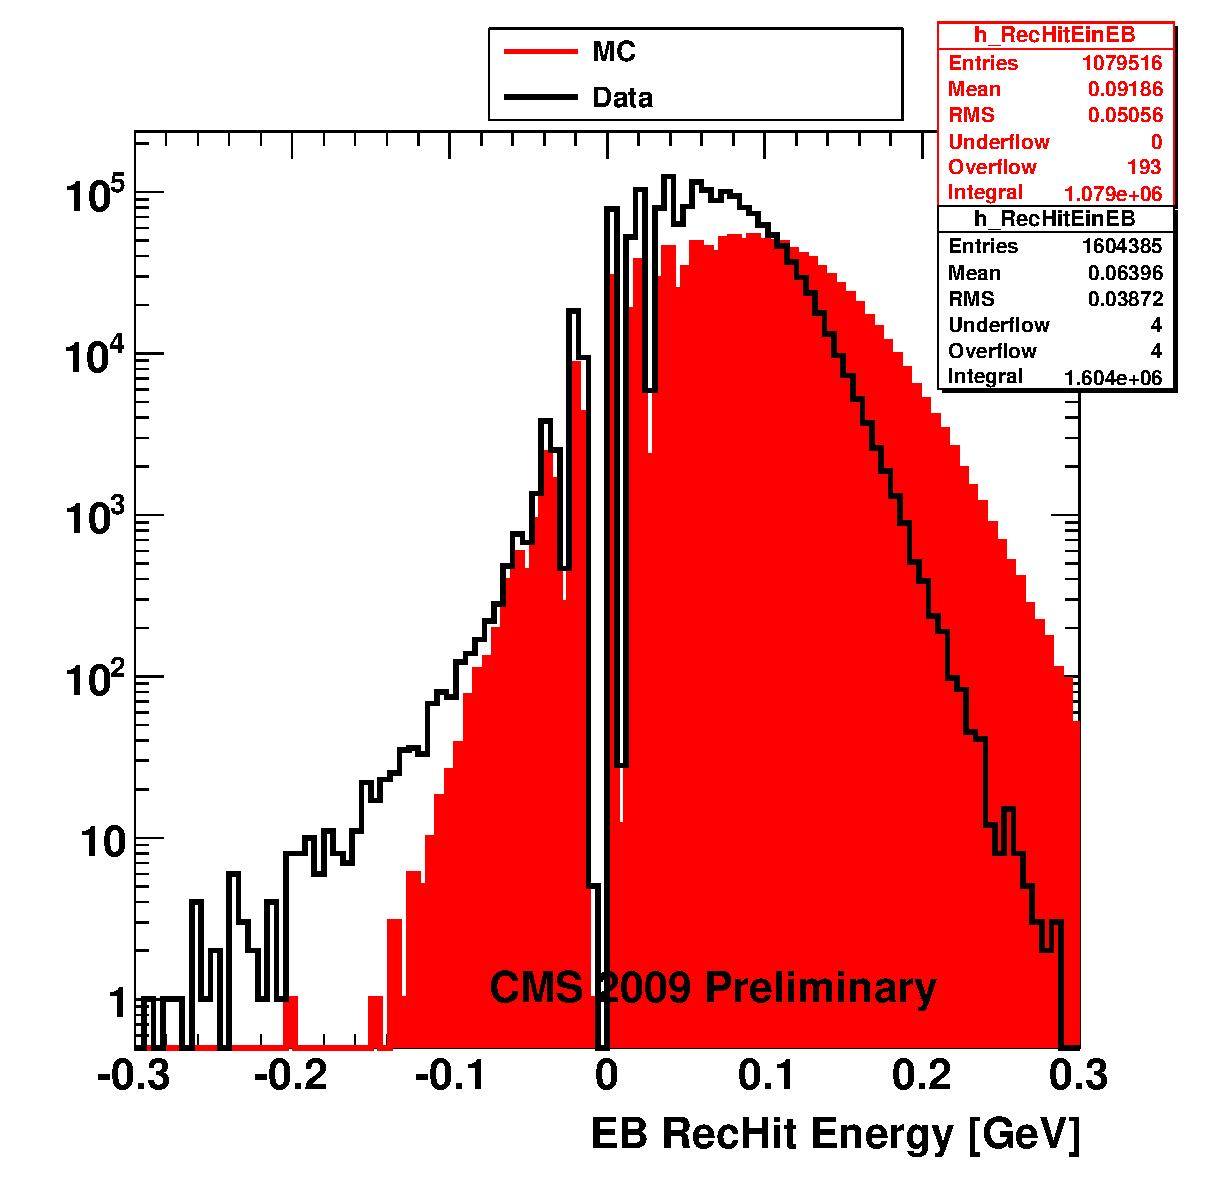
\includegraphics[width=0.33\textwidth]{plots_CaloNoise/h_RecHitEinEB.eps} &
  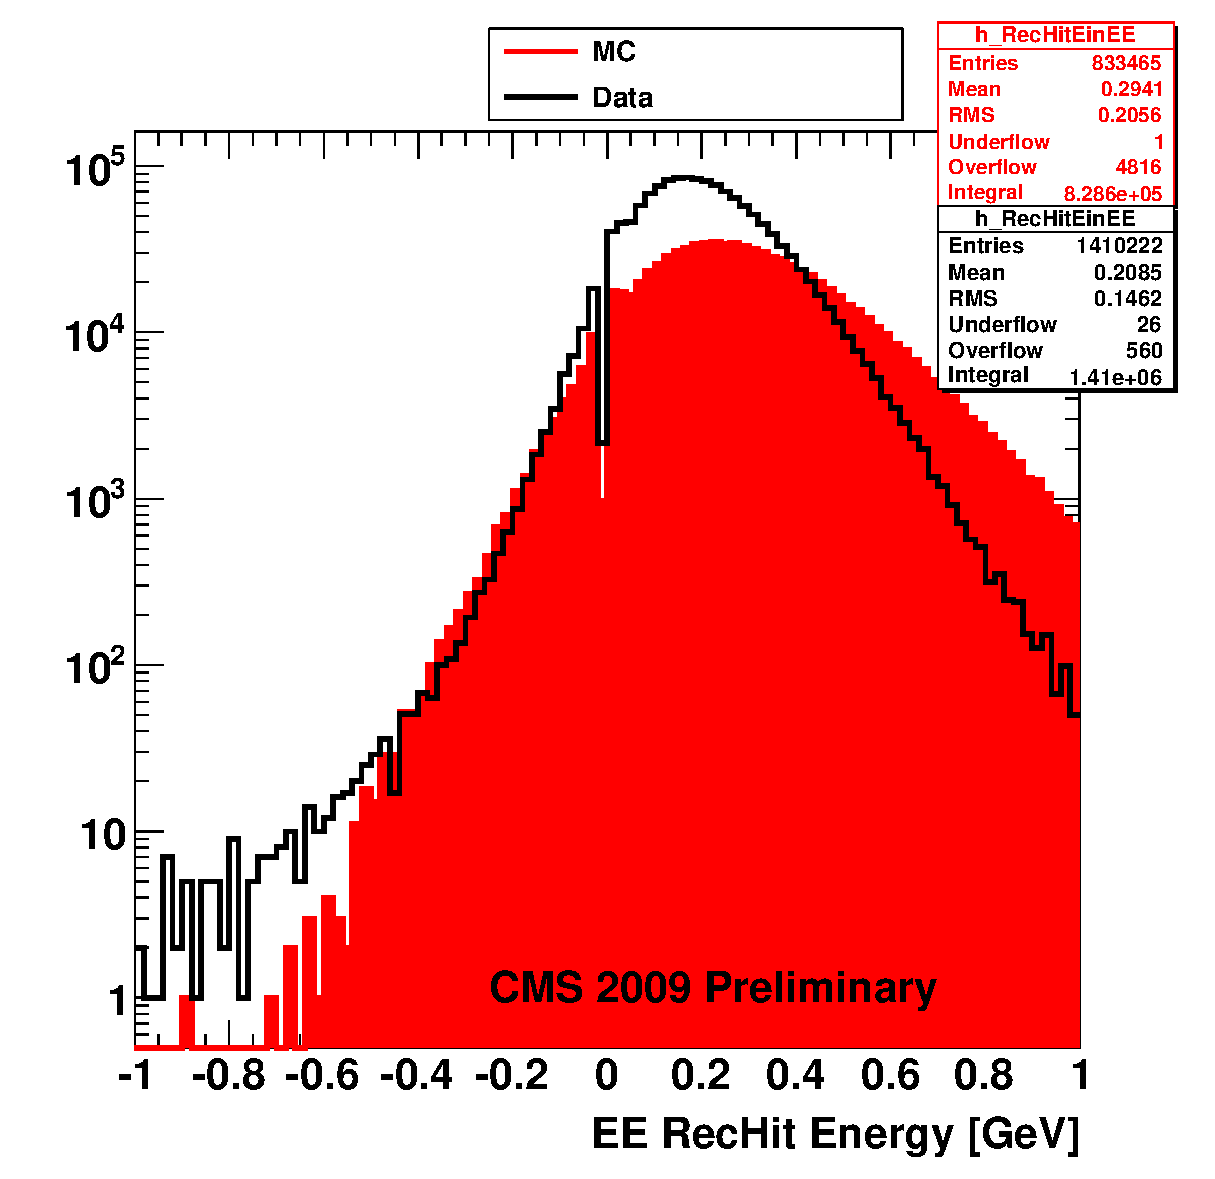
\includegraphics[width=0.33\textwidth]{plots_CaloNoise/h_RecHitEinEE.eps} \\
  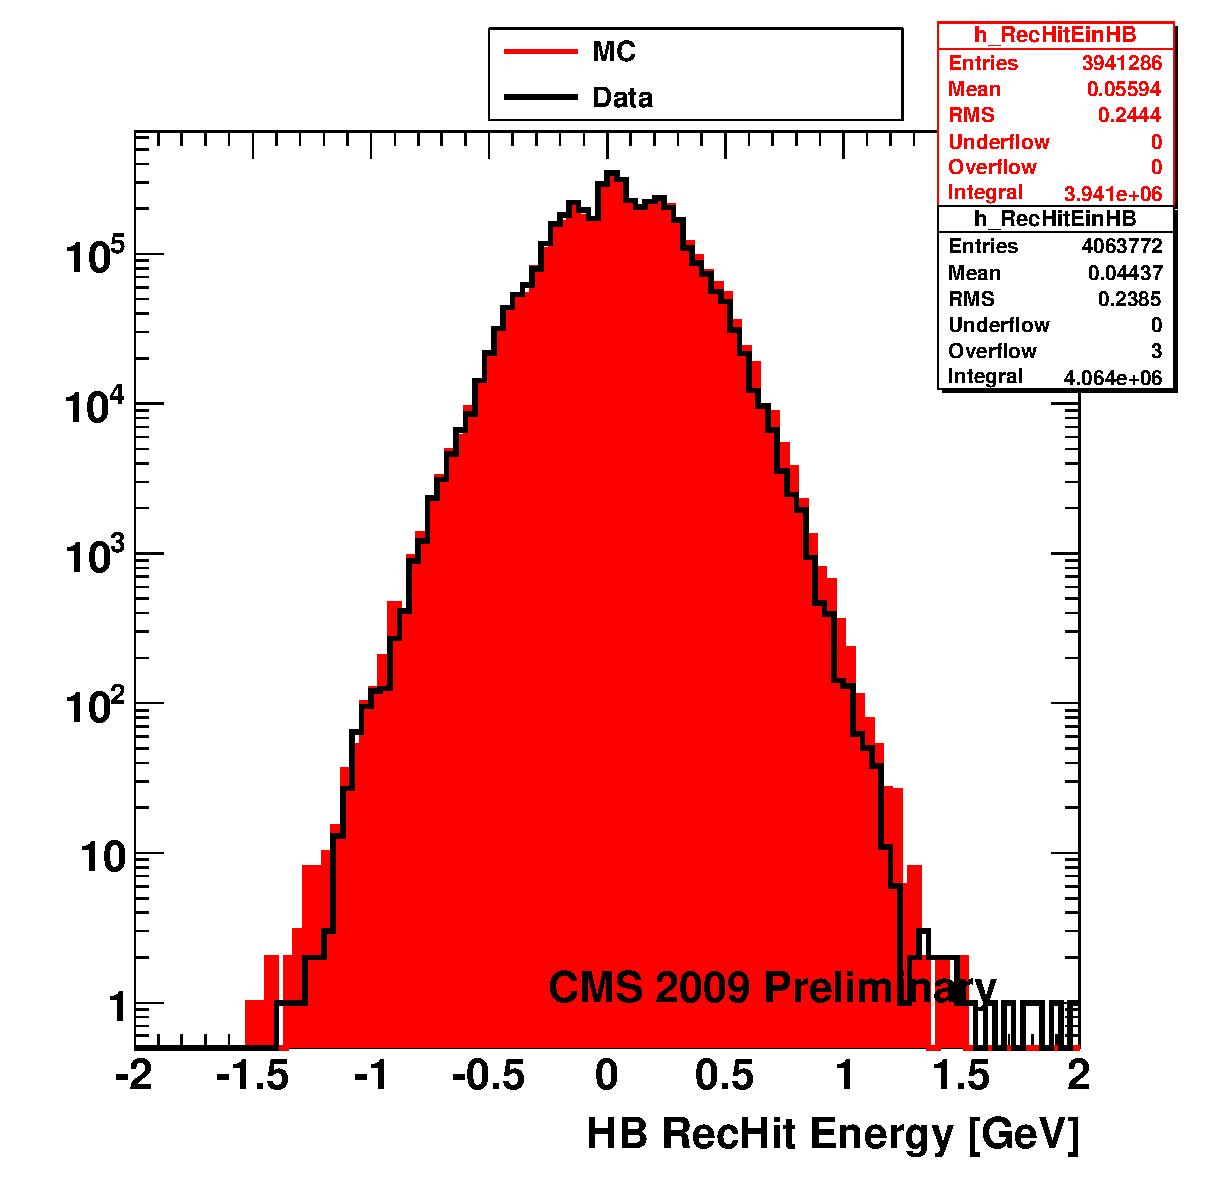
\includegraphics[width=0.33\textwidth]{plots_CaloNoise/h_RecHitEinHB.eps} &
  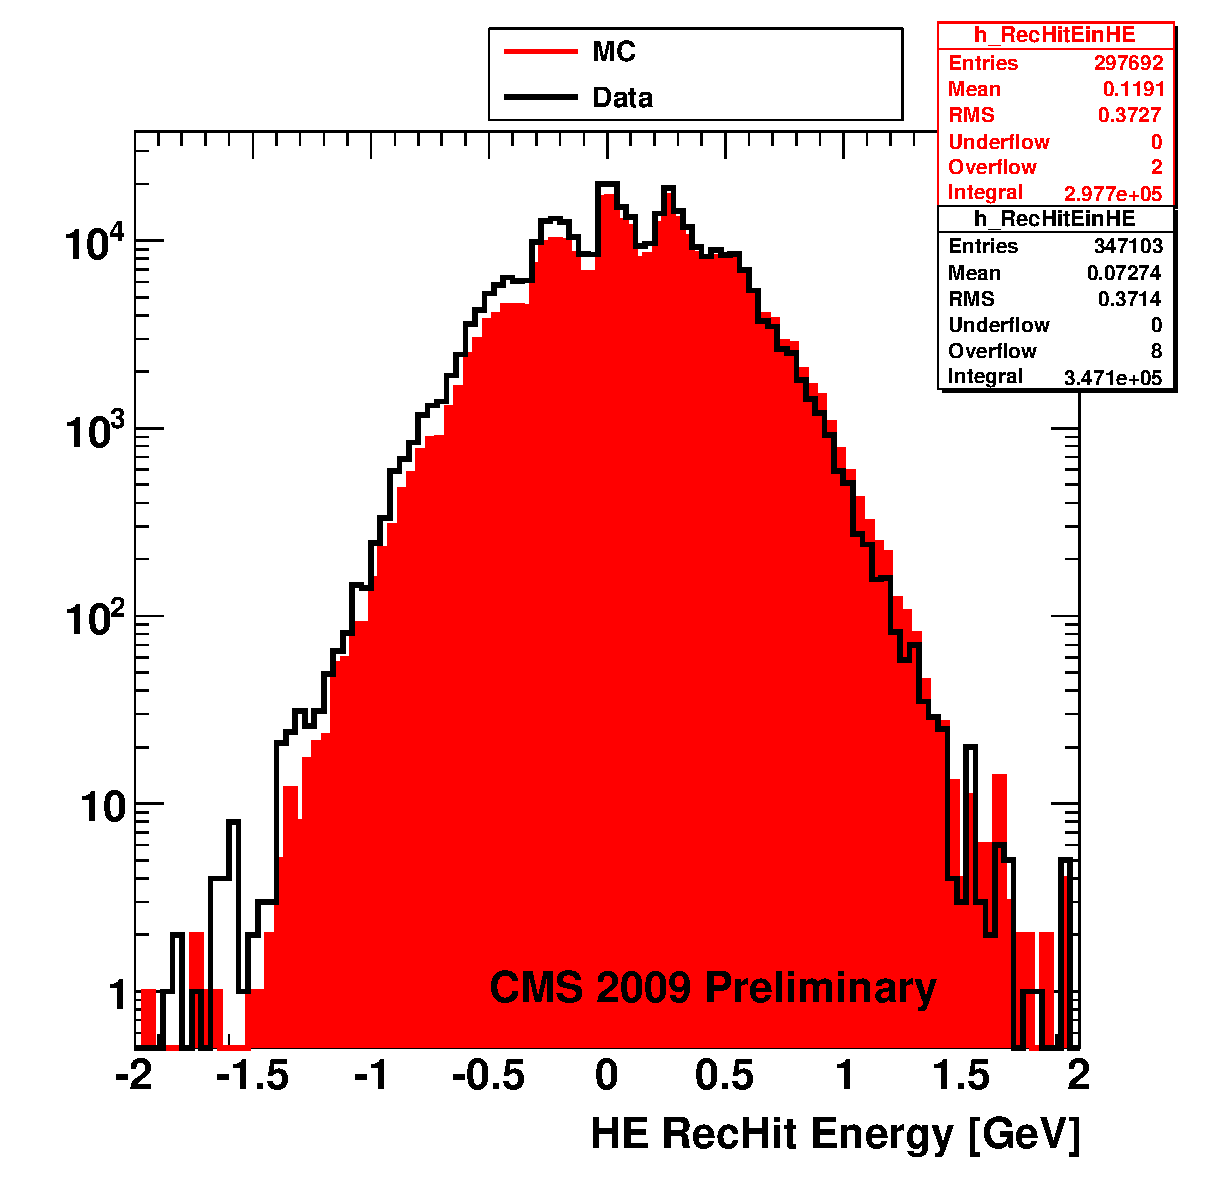
\includegraphics[width=0.33\textwidth]{plots_CaloNoise/h_RecHitEinHE.eps} \\
  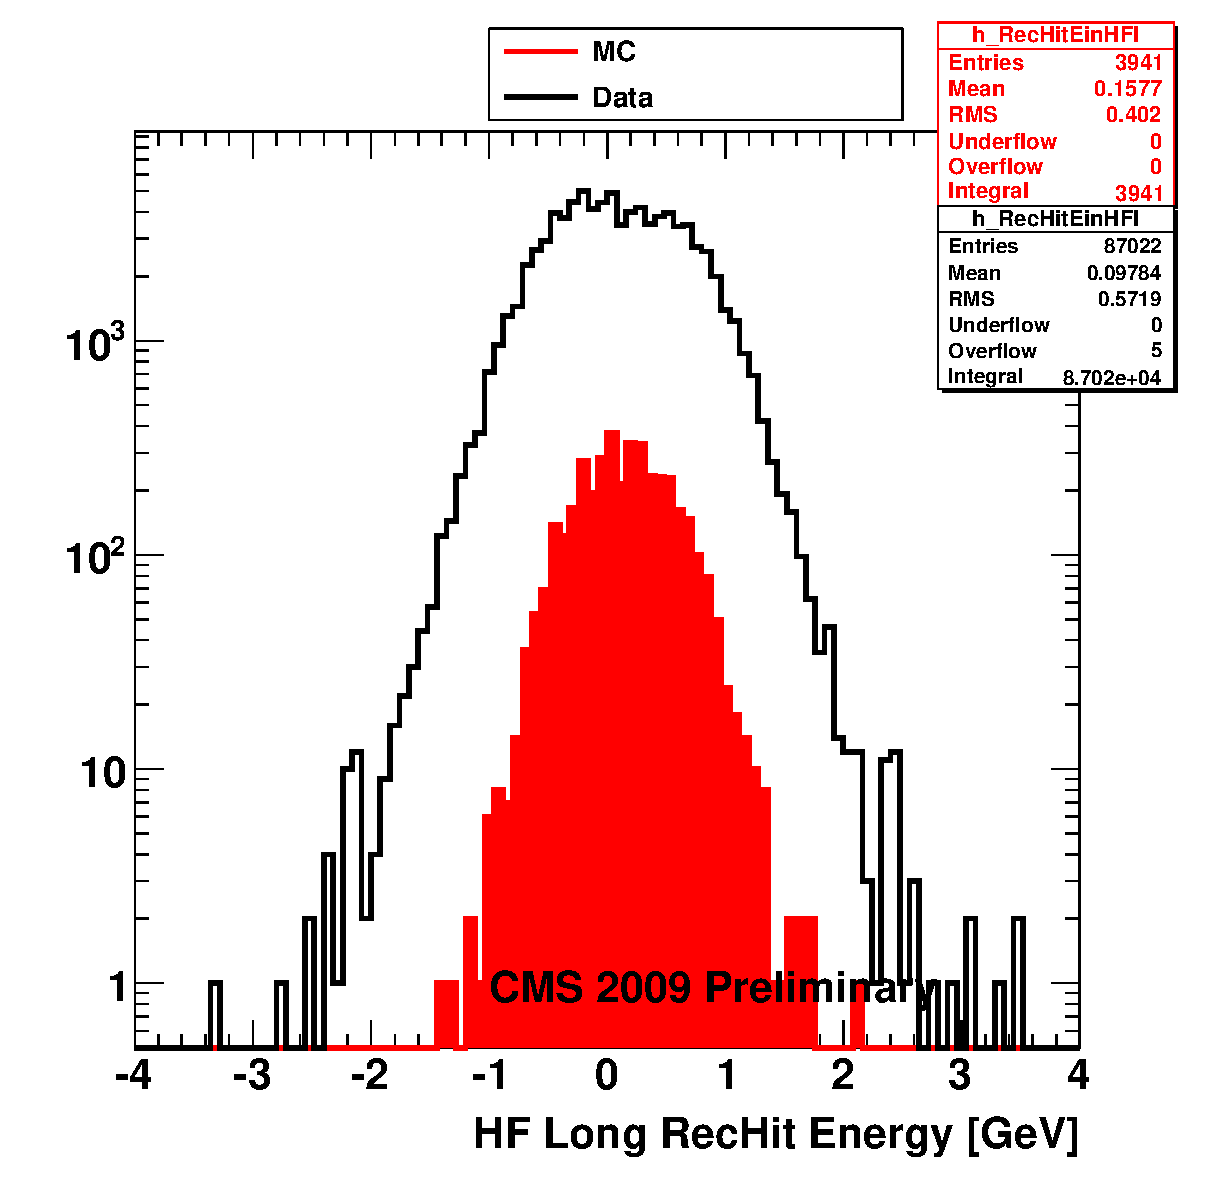
\includegraphics[width=0.33\textwidth]{plots_CaloNoise/h_RecHitEinHFl.eps} &
  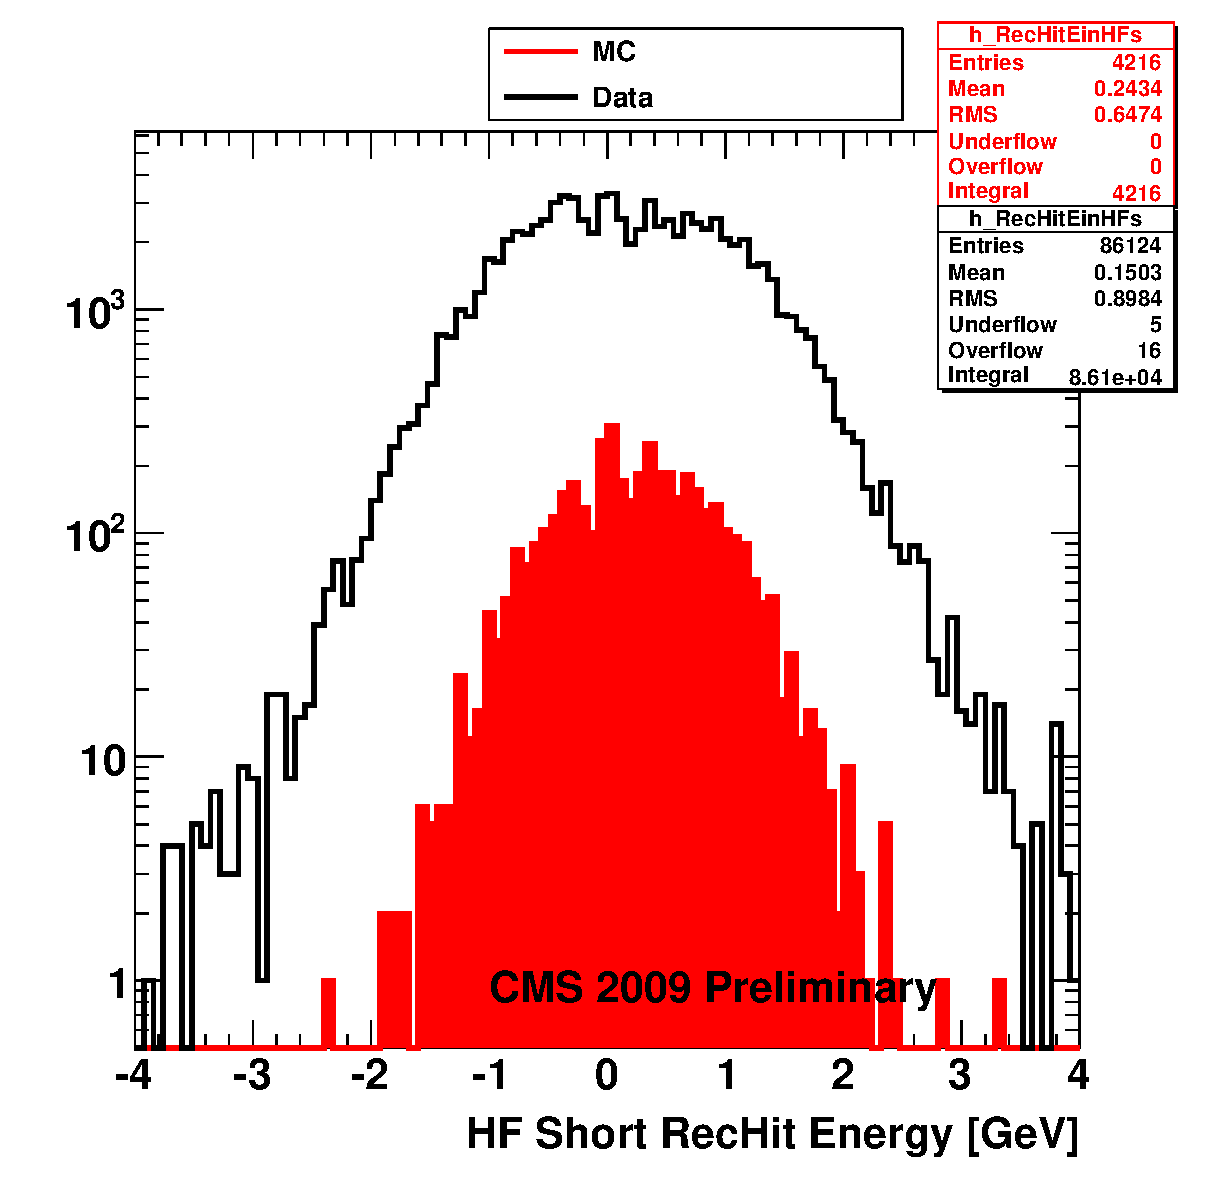
\includegraphics[width=0.33\textwidth]{plots_CaloNoise/h_RecHitEinHFs.eps} \\
 \end{tabular}
 \caption{\small RecHit energy distributions in noise-only (red-filled area) and selected ZeroBias data (black line) from
run 124022 for different calorimeter sub-detectors. The distributions shown are not normalized but correspond to the same number of events 
(5000 events).\label{fig:subdet_RecHitE}}
\end{figure}

\begin{figure}[h!]
 \centering
 \begin{tabular}{ll}
  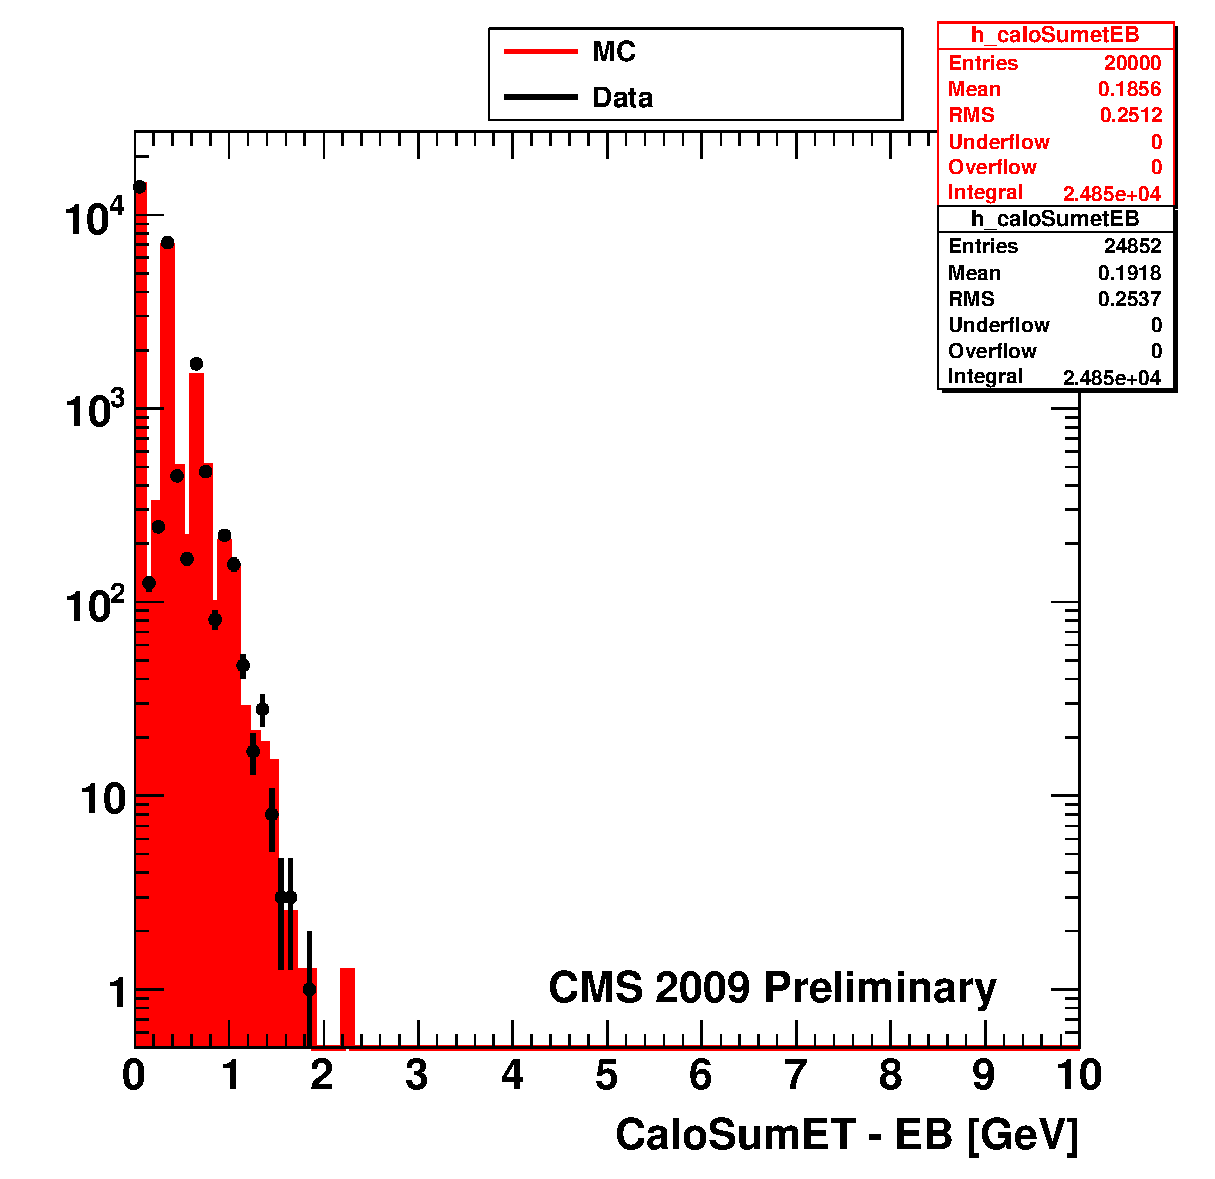
\includegraphics[width=0.33\textwidth]{plots_CaloNoise/h_caloSumetEB.eps} &
  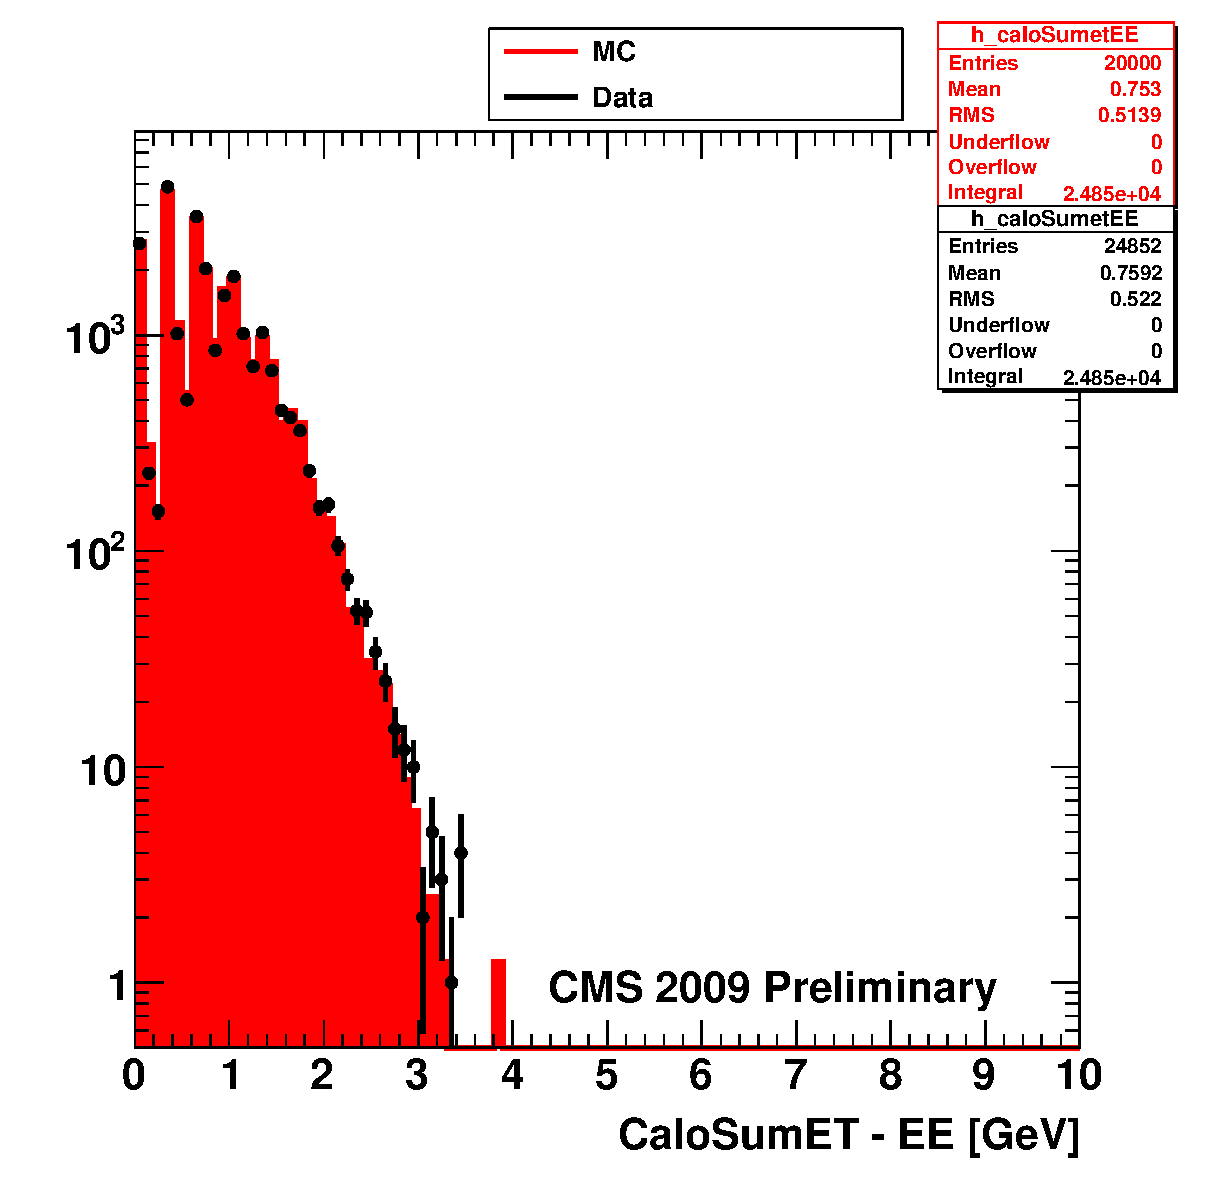
\includegraphics[width=0.33\textwidth]{plots_CaloNoise/h_caloSumetEE.eps} \\
  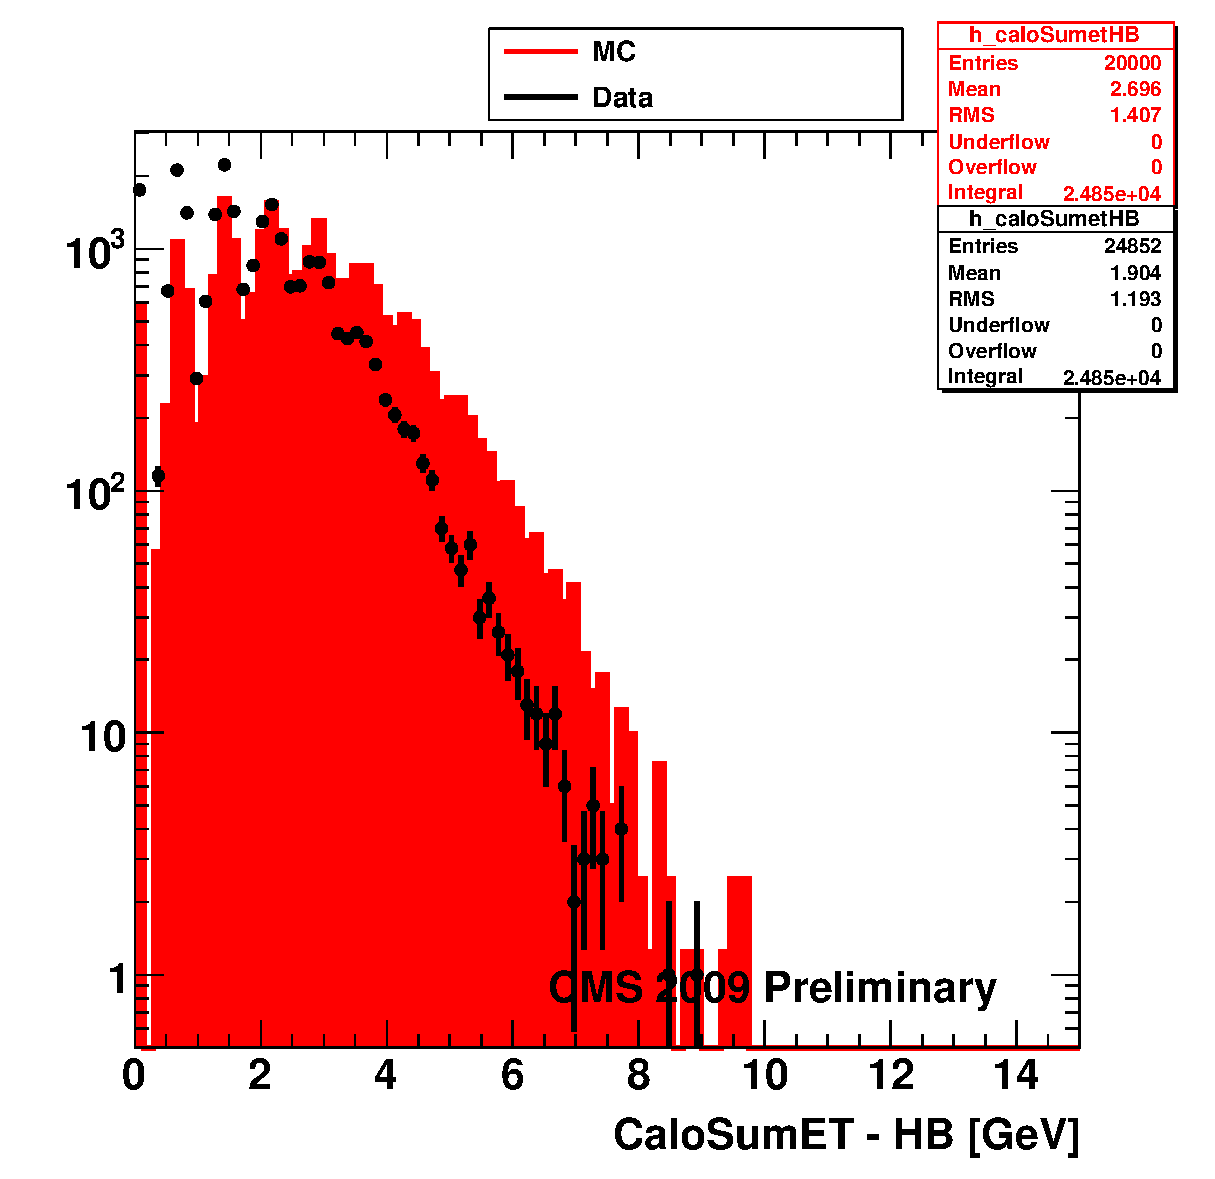
\includegraphics[width=0.33\textwidth]{plots_CaloNoise/h_caloSumetHB.eps} &
  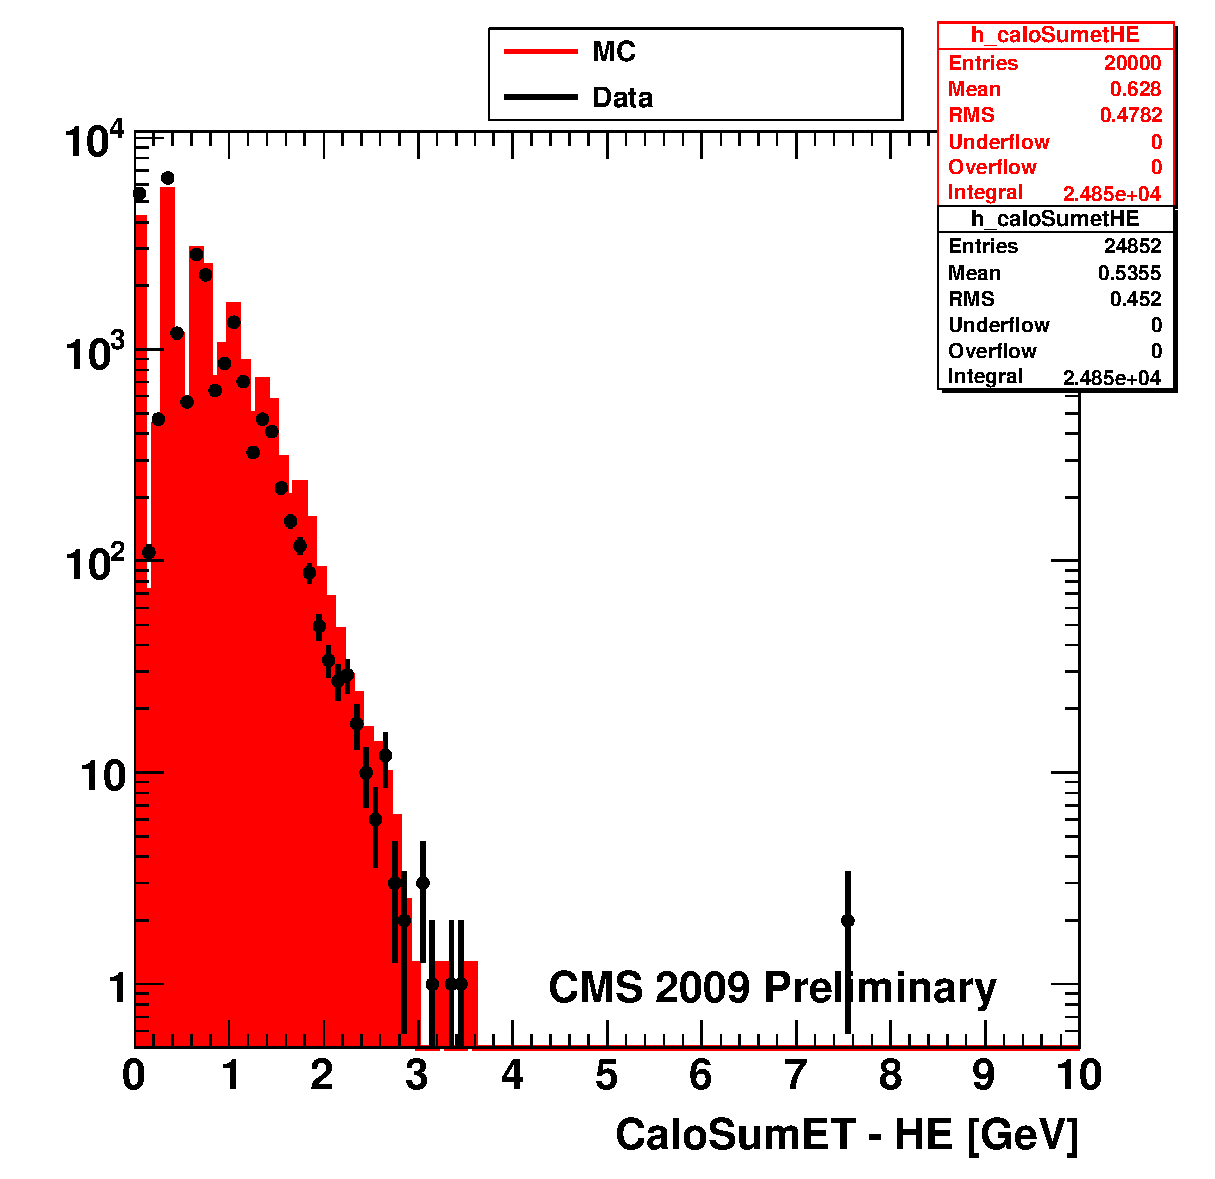
\includegraphics[width=0.33\textwidth]{plots_CaloNoise/h_caloSumetHE.eps} \\
  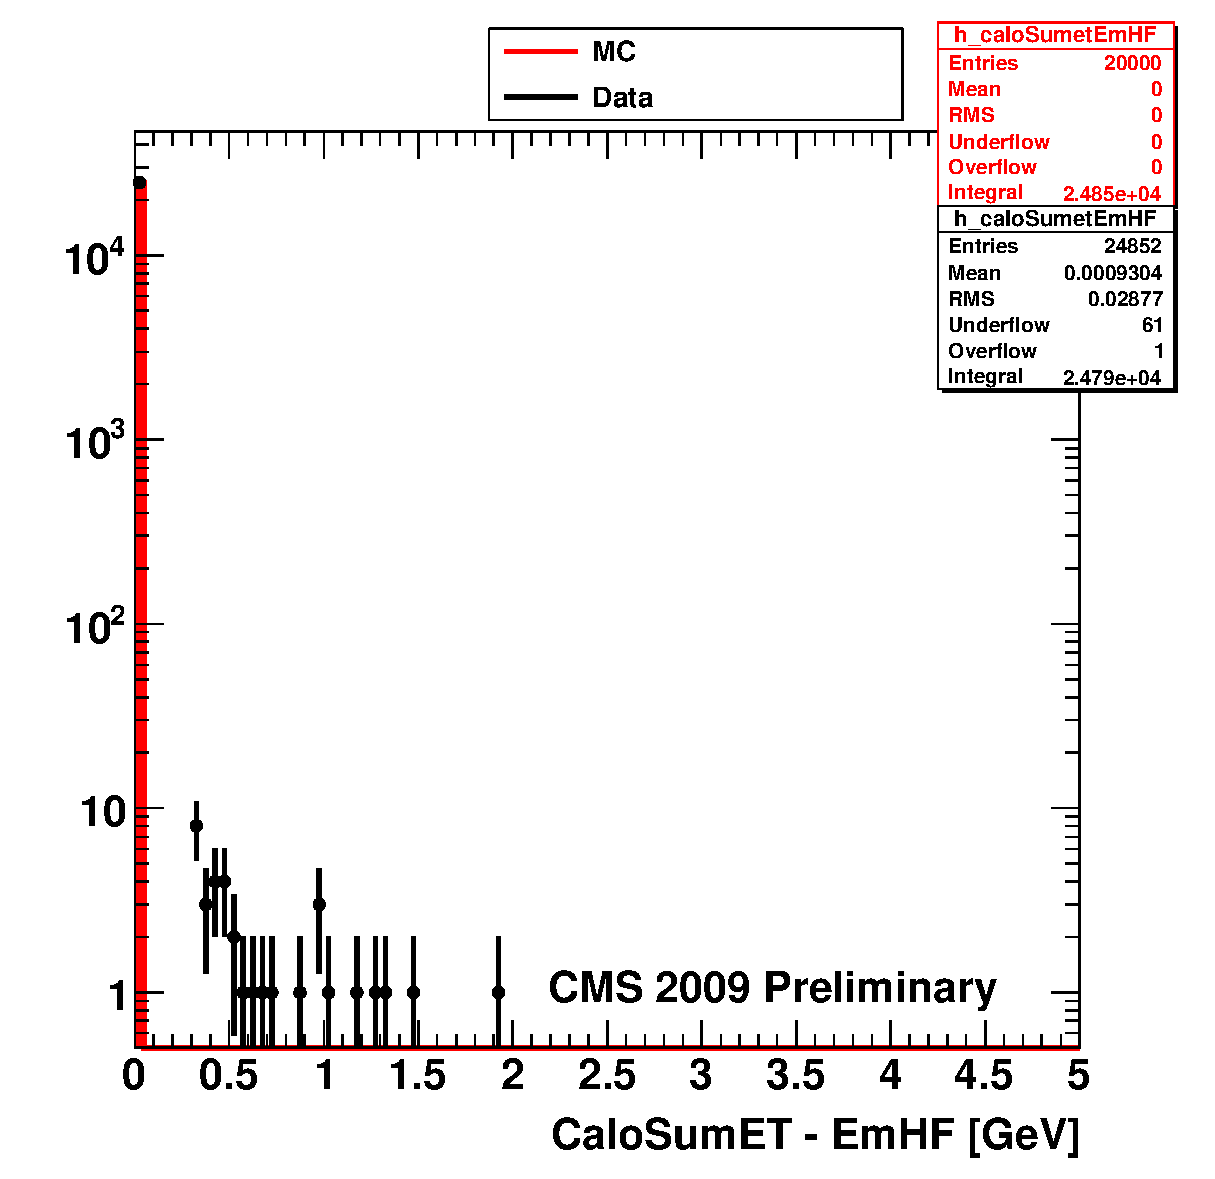
\includegraphics[width=0.33\textwidth]{plots_CaloNoise/h_caloSumetEmHF.eps} &
  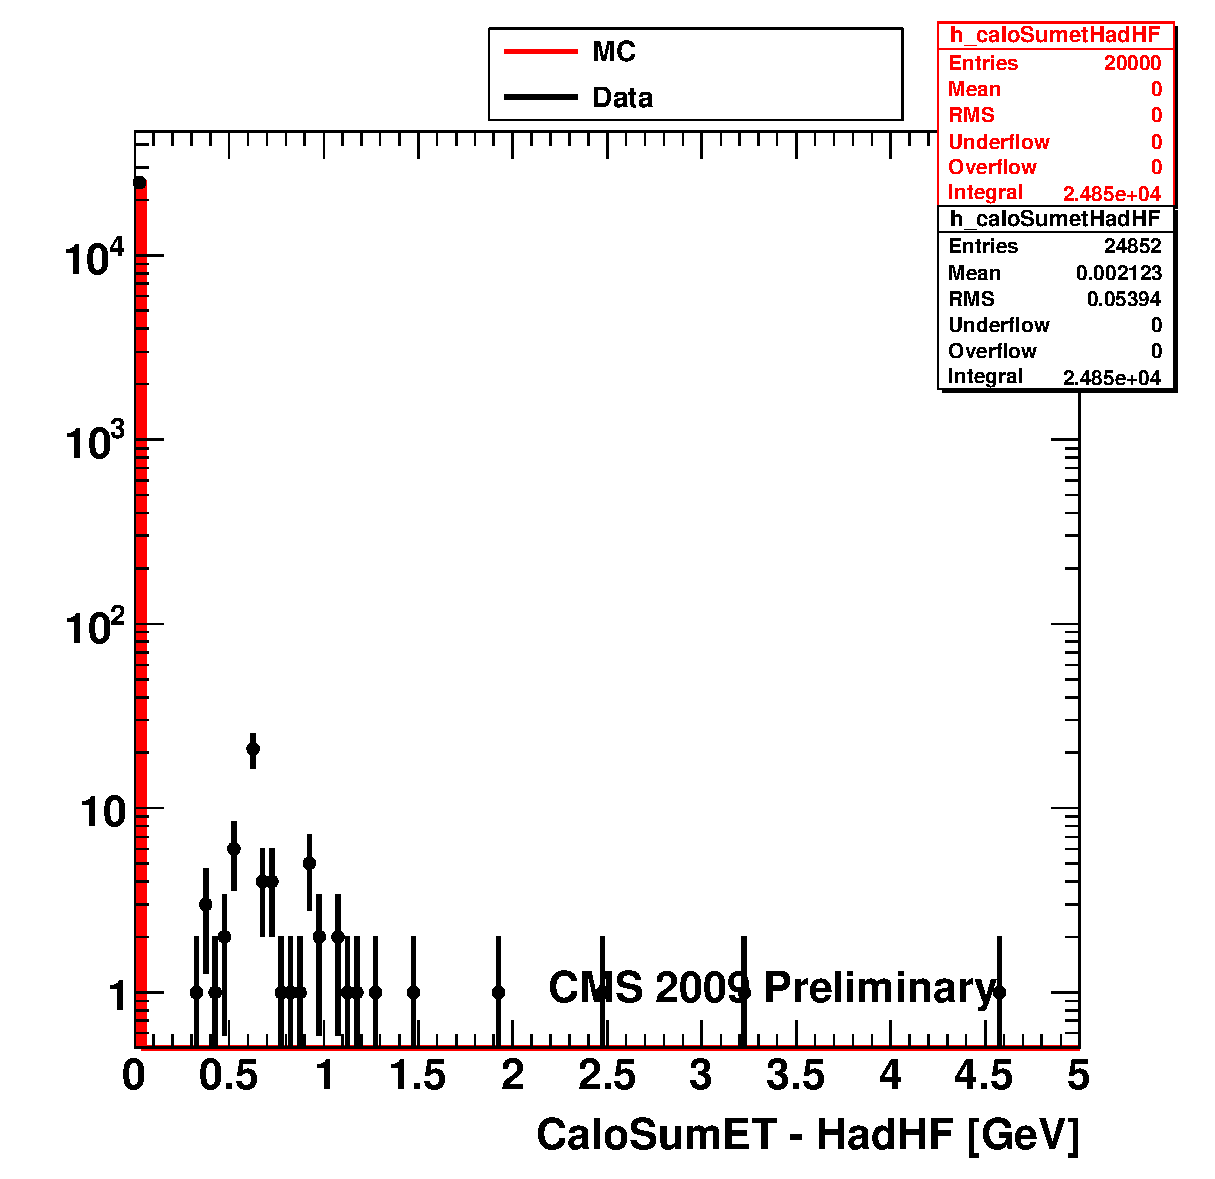
\includegraphics[width=0.33\textwidth]{plots_CaloNoise/h_caloSumetHadHF.eps} \\
 \end{tabular}
 \caption{\small CaloSumET distributions in noise-only (red-filled area) and selected ZeroBias data (black dots) from
run 124022 in different calorimeter sub-detectors. In the HF plots, entries outside the first bin correspond to the PMT
window hits.\label{fig:subdet_CaloSumET}}
\end{figure}

\clearpage
